\chapter{Tervez\'es}\label{chapter:tervezes}
Ebben a fejezetben a "WatchWithFriends" alkalmazás tervezési folyamatát mutatom be.
A fejezet első részében a felhasználói felület tervezését ismertetem,
majd a szerver és a kliens közötti kommunikáció megvalósítását.

\section*{Felhasználói felület tervezése}
FELHASZNÁLÓI FELÜLET!!!

\section*{Adatbázis}
\subsection*{ER modell egyedei és tulajdonságai}
\textbf{User-ek tulajdonságai:}
\begin{itemize}
    \item \underline{Id}: Elsődleges kulcs, Guid típusú.
    \item \underline{Name}: Felhasználó neve, szöveg típusú.
    \item \underline{Email}: Felhasználó email címe, szöveg típusú.
    \item \underline{PasswordHash}: Felhasználó jelszavának hash-elt változata, szöveg típusú.
    \item \underline{Salt}: Felhasználó jelszavának sója, szöveg típusú.
    \item \underline{BirthDate}: Felhasználó születési dátuma, dátum típusú.
\end{itemize}
\textbf{Image-ek tulajdonságai:}
\begin{itemize}
    \item \underline{Id}: Elsődleges kulcs, Guid típusú.
    \item \underline{Data}: Kép binárisa, byte tömb típusú.
\end{itemize}
\textbf{Room-ok tulajdonságai:}
\begin{itemize}
    \item \underline{Id}: Elsődleges kulcs, Guid típusú.
    \item \underline{Name}: Szoba neve, szöveg típusú.
    \item \underline{CreatorId}: Tulajdonos azonosítója, Guid típusú.
    \item \underline{CreationTime}: Szoba létrehozásának ideje, dátum típusú.
    \item \underline{CurrentVideoId}: Jelenleg lejátszott videó azonosítója, Guid típusú.
    \item \underline{PasswordHash}: Szoba jelszavának hash-elt változata, szöveg típusú.
    \item \underline{Salt}: Szoba jelszavának sója, szöveg típusú.
\end{itemize}
\textbf{Video-k tulajdonságai:}
\begin{itemize}
    \item \underline{Id}: Elsődleges kulcs, Guid típusú.
    \item \underline{Title}: Videó címe, szöveg típusú.
    \item \underline{Url}: Videó URL-je, szöveg típusú.
    \item \underline{ThumbnailURL}: Videó thumbnail-je, szöveg típusú.
\end{itemize}

\begin{figure}[H]
    \centering
    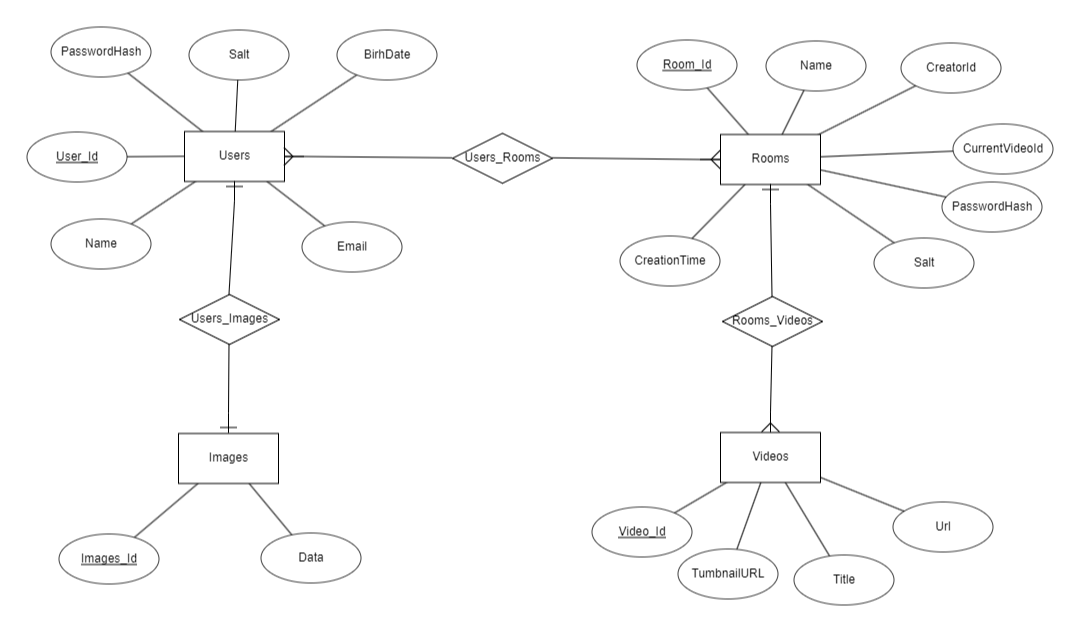
\includegraphics[width=15.0truecm]{images/er_modell.png}
    \caption{ER modell}
    \label{fig:er_modell}
\end{figure}

\subsection*{Relációs modell}
\textbf{Az egyedek közötti kapcsolatok:}
\begin{itemize}
    \item \underline{Users-Images}: 1:1 Egy felhasználóhoz tartozhat egy kép, és a kép csak egy fel-
          használóhoz.
    \item \underline{Users-Rooms}: N:N Egy felhasználóhoz tartozhat több szoba, egy szoba is tartozhat
          több felhasználóhoz.
    \item \underline{Room-Video}: 1:N Egy szobához tartozhat több videó, de egy videó csak egy
          szobához tartozhat.
\end{itemize}

\begin{figure}[H]
    \centering
    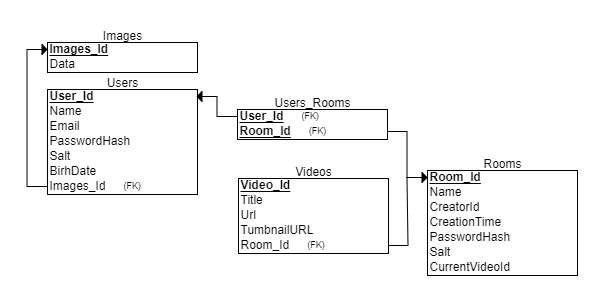
\includegraphics[width=15.0truecm]{images/relation_modell.png}
    \caption{Relációs modell}
    \label{fig:relation_modell}
\end{figure}

\section*{Szerver oldali logika}
\subsection*{Architektúra}
Az alkalmazásnál MVC (Model-View-Controller) architektúrára építettem, illetve
bővítettem a Repository és a Service rétegekkel. Az MVC architektúra egy
architektúrális minta, amely a felhasználói felületet (View), az alkalmazás
logikáját (Controller) és az adatokat (Model) három különálló részre osztja.
A Repository réteg a Model réteghez tartozik, a Service réteg pedig a Controller réteghez.
Azért bontottam tovább a rétegeket, mert így jobban elkülönülnek a felelősségi körök,
és a kód is átláthatóbb lesz, illetve könnyebben bővíthető, és tesztelhető lesz.
\\
\\
\begin{figure}[H]
    \centering
    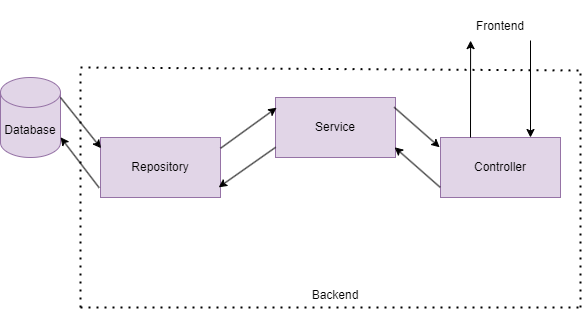
\includegraphics[width=14.0truecm]{images/Backend_architecture.png}
    \caption{Backend Architektúra}
    \label{fig:backend_architecture}
\end{figure}
\textbf{Ismertetem a rétegek főbb tulajdonságait:}
\begin{itemize}
    \item \textbf{Adatbázis}: Az alkalmazásom adattára. Itt tárolódnak a statikus és dinamikus adatok.
    \item \textbf{Repositoryk}: Az adatbázis és az alkalmazás logikája közötti köztes réteg. CRUD műveletek, komplex lekérdezések.
    \item \textbf{Servicek}: Az üzleti logika helye. Itt történnek a komplex számítások, validációk és egyéb logikai műveletek.
    \item \textbf{Controllerek}: Az API végpontokat kezelő réteg. Fogadják a kliens kéréseit, és válaszokat generálnak.
\end{itemize}

\subsection*{Szoftvertervezési elvek (tervezés)}
A szoftvertervezési elvek alapvető útmutatások a kiváló kód fejlesztéséhez. Ezek az iránymutatások növelik a kód minőségét, gyorsítják a fejlesztési folyamatot és minimalizálják a hibalehetőségeket. Az ilyen elvek segítenek abban, hogy a kód könnyen újrafelhasználható és karbantartható legyen.

A kód olvashatóságát és tesztelhetőségét is javítják, ami hosszú távon időt és erőforrást spórol. A rugalmasság és a bővíthetőség is nő, tehát a kód könnyen adaptálható új funkciók vagy változások esetén. Továbbá, ezek az elvek ösztönzést nyújtanak a kódbázis redundancia kiküzsöbölésére, amely csökkenti a komplexitást és növeli a kohéziót. Az elvek célja a kód moduláris felépítése és az alacsonyabb összekapcsoltság, ami hozzájárul a jobb szervezettséghez és könnyebb karbantartáshoz.

Összességében, a szoftvertervezési elvek olyan iránymutatások, amelyek célja a hatékony, karbantartható és minőségi kód létrehozása.
A szoftver implementációja során a SOLID elveket vettem alapul.

\section*{UML diagram}

\begin{figure}[H]
    \centering
    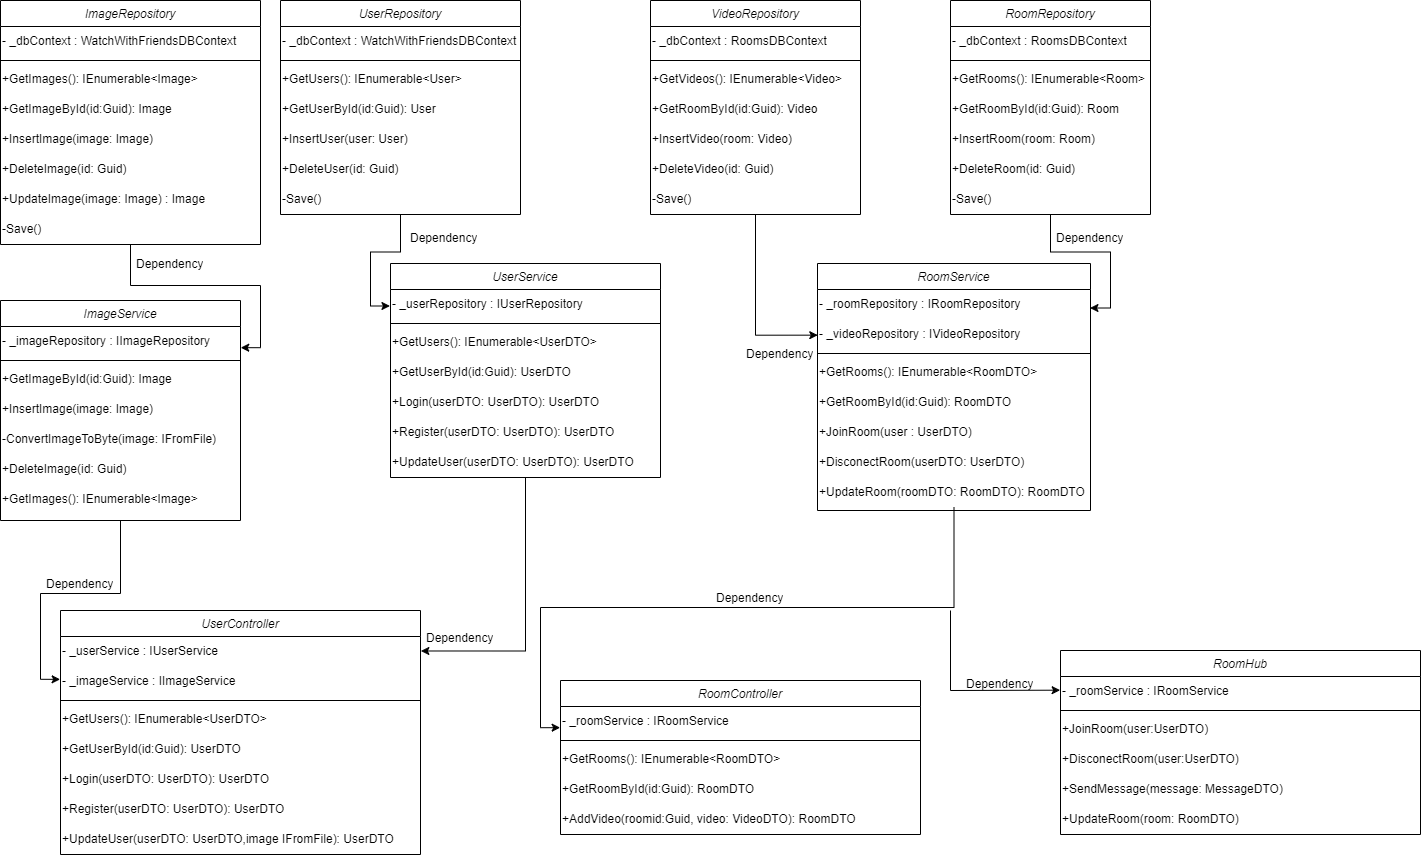
\includegraphics[width=14.0truecm]{images/UML_Diagram.png}
    \caption{UML Diagram}
    \label{fig:uml_diagram}
\end{figure}

Az architektúra alapját egy kibővített MVC (Model-View-Controller) rendszer adja,
amely kifinomult kapcsolatokat biztosít az egyes szerveroldali osztályok között. Mivel a back-end és a front-end kapcsolata indirekt,
ezért a megjelenítési oldalon található logika nincs semmilyen ráhatással a szerver struktúrális felépítésére.
Ebben az elrendezésben az egyes osztályok nem csak az alapvető CRUD (Create,
Read, Update, Delete) műveletekért felelnek, hanem a komplex üzleti logika egyedi
implementációját is lehetővé teszik. Az adatmodell és a kontroller között az adatátviteli objektumok (DTO-k) és a repository minták segítenek a moduláris és tiszta kód

struktúra fenntartásában. A repository-k pedig közvetlenül a dedikált adatbázis-kontextusokhoz kapcsolódnak.

A kapcsolatok közötti szoros integráció lehetővé teszi az adatok egyszerű és követke-
zetes kezelését, miközben fenntartja a kód karbantarthatóságát és tesztelhetőségét. Az

egész rendszer ezen az elrendezésen alapul, így garantálva, hogy a szerveroldali logika
jól szervezett és hatékony maradjon.